\section{Manual for the software control of the morbidostat}

This section describes how to switch on specific pumps which is important for disinfecting the morbidostat and how to start morbidostat experiments. First we need to understand the layout of the pumps and how they are assigned. As shown in Figure \ref{figure:pump_layout} 9 pump boxes with five pumps are responsible for injecting antibiotics and media in 15 vials. Every pump box is connected with a numbered connector to the microcontroller. The first layer of pump boxes (connector one, two, three) is named pump1 and connected to media. The second layer (connector four, five, six) is named pump2 and connected to a low-concentrated antibiotic. The top layer (connector seven, eight, nine) is named pump3 and connected to a high-concentrated antibiotic. Within a pump box, every pump has a number as well. The designed layout implies that within one layer of pumps, the individual pumps were numbered from zero to 14. Because the pumps were connected column by column, the same pump number of every box is responsible for injecting fluids in the according vial. Because the pump layout was implemented with zero indexing, the pump number is shifted by one compared to the vial number. \textit{E.g.} P\_0 from pump1, P\_0 from pump2 and P\_0 from pump3 are responsible for injecting media and antibiotics into vial 1. 
\begin{figure}[H]
	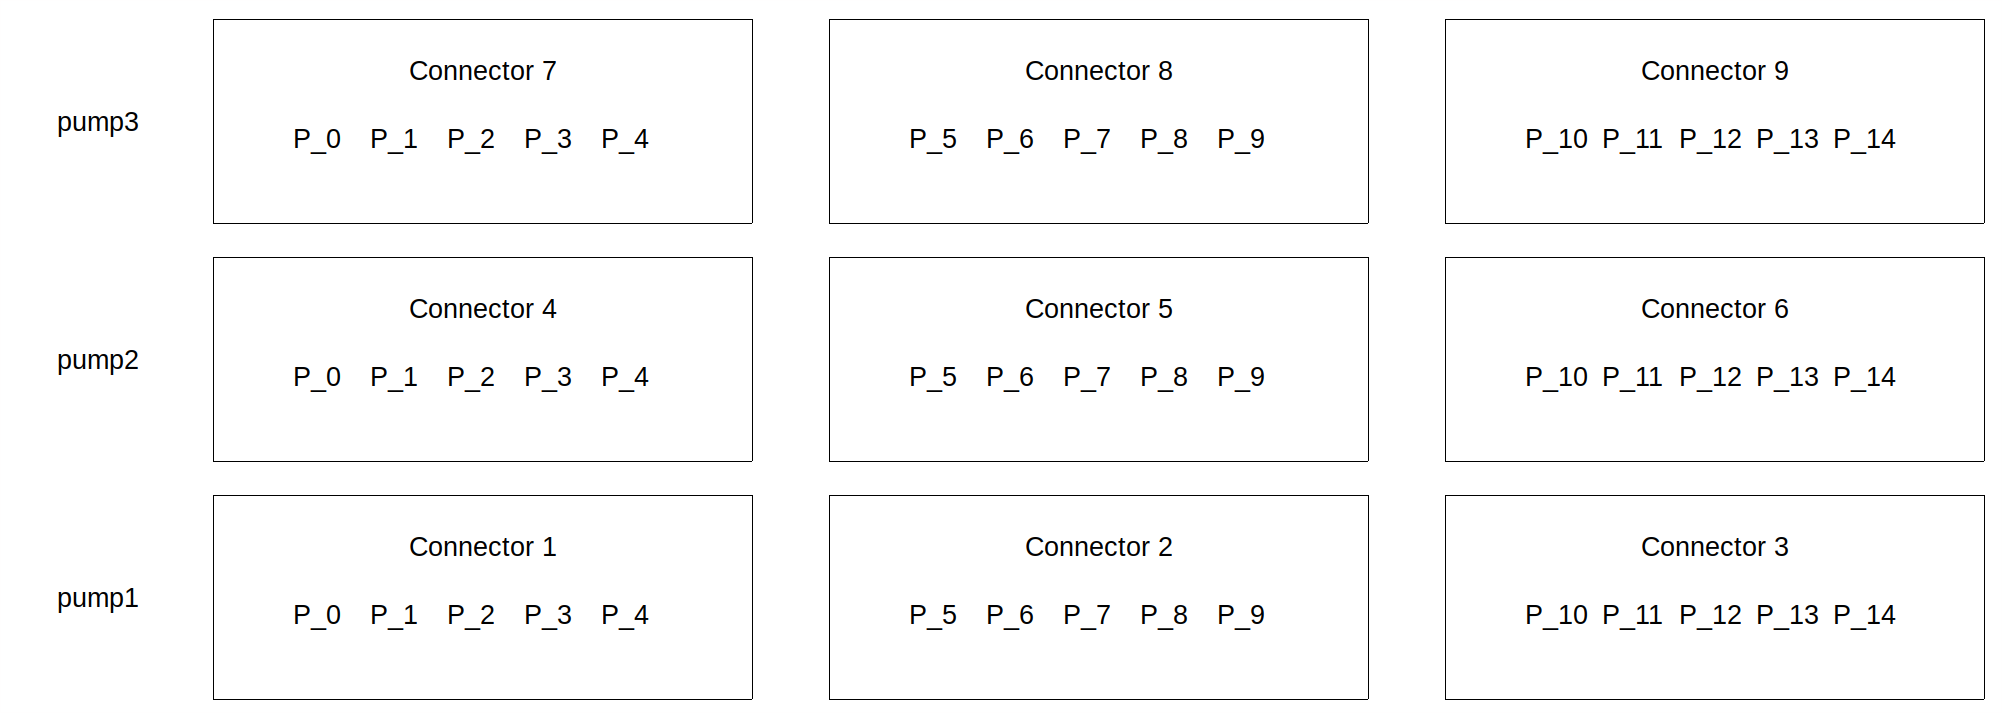
\includegraphics[width=1\textwidth]{pump_mapping.png}
	\caption{Pump layout of the pump stacks. P\_N stands for the pump number.}
	\label{figure:pump_layout}
\end{figure}
\subsection{Manually turning on pumps of the morbidostat}
Manual control of the morbidostat is possible by running \href{https://github.com/nahanoo/ESBL\_project/}{morbidostat\_experiment.py} in the interactive IPython mode. Therefore, open the terminal and navigate to the location of the \href{https://github.com/nahanoo/ESBL\_project/}{morbidostat\_experiment.py} file.
\begin{verbatim}
cd /home/python_morbidostat/python_src
\end{verbatim} 
Run \href{https://github.com/nahanoo/ESBL\_project/}{morbidostat\_experiment.py} in the interactive python mode and initialize the morbidostat. For initializing the morbidostat we need to pass the vial numbers that we want to use to the morbidostat as a list. Indexing starts at zero again. In this example we initialized the morbidostat with the first ten vials. 
\begin{verbatim}
ipython morbidostat_experiment.py --i
morb = morbidostat(vials=[0,1,2,3,4,5,6,7,8,9,10])
\end{verbatim}
Within IPython we can call various functions. The following code shows examples of functions for turning on pumps. Text followed by \# are comments and not relevant for the functions.
\begin{verbatim}
morb.run_all_pumps('pump1',30)	# Run all pumps of the first 
layer pump1 for 30 seconds
morb.morb.run_pump('pump1,0,30)	# Run P_0 from pump1 for 30 seconds
morb.morb.inject_volume('pump1',0,10)	# Inject 10 mL in P_0 from pump1
morb.morb.run_waste_pump(30) # Run waste pump for 30 seconds
morb.morb.remove_waste(10)		# Remove 10 mL of waste from all the vials
\end{verbatim}

\subsection{Staring morbidostat experiments}
For starting morbidostat experiments we created a template in a csv file. In this csv file we can specify which vials we want to use for our experiments in which mode. Additionally, we need to specify a few values, mainly important for the continuous mode. We can define which concentrations of the antibiotics we use, which target\_OD we would like to approximate, the dilution factor and the MIC of the strains used for the experiment. To edit the template, open the csv file /home/morbidostat/python\_morbidostat/setup.csv
\begin{figure}[H]
	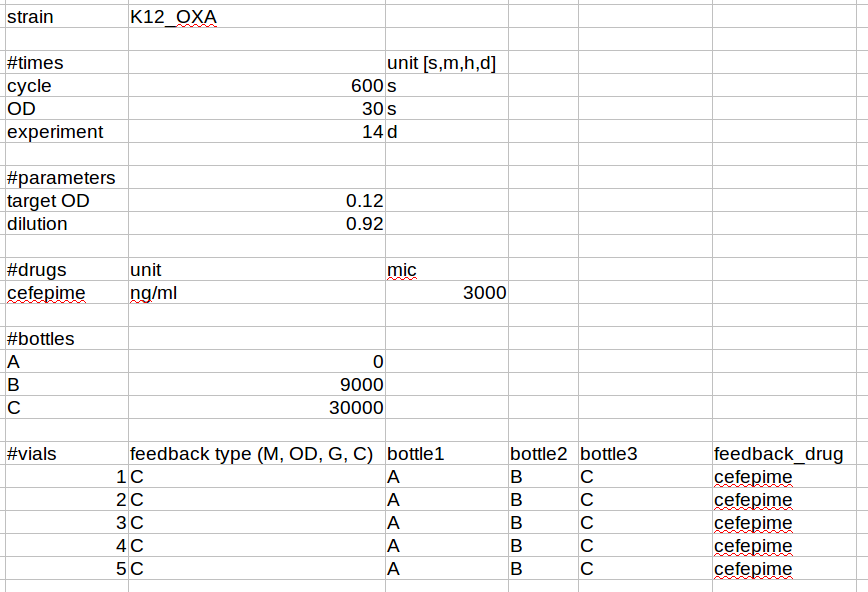
\includegraphics[width=1\textwidth]{template.png}
	\caption{Template used to start morbidostat experiments. In the column namend vials you can enter which vials you want to use for the experiment. Indexing starts at 1. Bottle1 is mapped to pump1, bottle2 to pump2, and bottle3 to pump3.}  
\end{figure}
After you edited the template you must save it. In the same directory a bash script called experiment\_from\_table.sh is located. We can use this script to start experiments based on our template. 
Execute the script by typing:
\begin{verbatim}
./experiment_from_table.se setup.csv
\end{verbatim}
Now the morbidostat experiment is running. You can always change parameters defined in the template while the morbiodstat is running. Here are some useful commands while the morbiodstat is running.
\begin{verbatim}
morb.dilution_factor = x	# Change the dilution factor 
morb.target_OD = x			# Change the target_OD
morb.cycle_dt = # 			# Change the cycle time
morb.interrupt_experiment()	# Interrupt the experiment. Necessary if you 
want to change the bottles with media or antibiotics
morb.resume_experiment() 	# Resume the experiment
morb.stop_experiment()		# Stops the experiment
morb.drug_concentrations[2][0] = x # Change the drug concentration of bottle2
morb.drug_concentrations[1][0] = x # Change the drug concentration of bottle3
morb.mics[0] = x 			# Change the mic of the strain
morb.reset_concentrations()	# Sets drug concentration in the vials to
0, imprtant if you transfer into a new vial
\end{verbatim}




\label{section:manual}

\section{Gibson cloning}
\subsection{Sequences of fragments}
\label{section:sequences}
ID: pEU22 \\ \DNA!GCCCACAGAATGATGTCACGCTGAAAATGCCGGCCTTTGAATGGGTTCATGTGCAGCTCCATCAGCAAAAGGGGATGATAAGTTTATCACCACCGACTATTTGCAACAGTGCCCTGAAAACTATATCAAAGAAGCCAAATACGACATGGCGGTGGGTCATCTCTTGCTAAAGTCATTTTGGGCGAATGAAGCCGTGTTTCAAATGATGATGCTTTCATATAACCTATTTTTGTTGTTCAAGTTTGATTCCTTGGACTCTTCAGAATACAGACAGCAAATAAAGACCTTTCGTTTGAAGTATGTATTTCTTGCAGCAAAAATAATCAAAACCGCAAGATATGTAATCATGAAGTTGTCGGAAAACTATCCGTACAAGGGAGTGTATGAAAAATGTCTGGTATAATAAGAATATCATCAATAAAATTGAGTGTTGCTCTGTGGATAACTTGCAGAGTTTATTAAGTATCATTGCAGCAAAGATGAAATCAATGATTTATCAAAAATGATTGAAAGGTGGTTGTAAATAATGTTACAATGTGTGAGAAGCAGTCTAAATTCTTCGTGAAATAGTGATTTTTGAAGCTAATAAAAAACACACGTGGAATTTAGGGACTATTCATGTTGTTGTTATTTCGTATCTTCCAGAATAAGGAATCCC'{red}ATGGTTAAAAAATCACTGCGCCAGTTCACGCTGATGGCGACGGCAACCGTCACGCTGTTGTTAGGAAGTGTGCCGCTGTATGCGCAAACGGCGGACGTACAGCAAAAACTTGCCGAATTAGAGCGGCAGTCGGGAGGCAGACTGGGTGTGGCATTGATTAACACAGCAGATAATTCGCAAATACTTTATCGTGCTGATGAGCGCTTTGCGATGTGCAGCACCAGTAAAGTGATGGCCGCGGCCGCGGTGCTGAAGAAAAGTGAAAGCGAACCGAATCTGTTAAATCAGCGAGTTGAGATCAAAAAATCTGACCTTGTTAACTATAATCCGATTGCGGAAAAGCACGTCAATGGGACGATGTCACTGGCTGAGCTTAGCGCGGCCGCGCTACAGTACAGCGATAACGTGGCGATGAATAAGCTGATTGCTCACGTTGGCGGCCCGGCTAGCGTCACCGCGTTCGCCCGACAGCTGGGAGACGAAACGTTCCGTCTCGACCGTACCGAGCCGACGTTAAACACCGCCATTCCGGGCGATCCGCGTGATACCACTTCACCTCGGGCAATGGCGCAAACTCTGCGGAATCTGACGCTGGGTAAAGCATTGGGCGACAGCCAACGGGCGCAGCTGGTGACATGGATGAAAGGCAATACCACCGGTGCAGCGAGCATTCAGGCTGGACTGCCTGCTTCCTGGGTTGTGGGGGATAAAACCGGCAGCGGTGGCTATGGCACCACCAACGATATCGCGGTGATCTGGCCAAAAGATCGTGCGCCGCTGATTCTGGTCACTTACTTCACCCAGCCTCAACCTAAGGCAGAAAGCCGTCGCGATGTATTAGCGTCGGCGGCTAAAATCGTCACCGACGGTTTG ! \\
Sequence coding for \textbeta-lactamase CTX-M-1 marked in red. The sequence was extracted from patient 25 sample 1. \\

ID: pEU23:\\
\DNA!GTGATCCCCTGGGCGAAATGCGCCTGGTAAGCAGAGTTTTTGAAATGTAAGGCCTTTGAATAAGACAAAAGGCTGCCTCATCGCTAACTTTGCAACAGTGCCTTTAAGCGTGCATAATAAGCCCTACACAAATTGGGAGTTAGACATCATGAGCAACGCAAAAACAAAGTTAGGCATCACAAAGTACAGCATCGTGACCAACAGCAACGATTCCGTCACACTGCGCCTCATGACTGAGCATGACCTTGCGATGCTCTATGAGTGGCTAAATCGATCTCATATCGTCGAGTGGTGGGGCGGAGAAGAAGCACGCCCGACACTTGCTGACGTACAGGAACAGTACTTGCCAAGCGTTTTAGCGCAAGAGTCCGTCACTCCATACATTGCAATGCTGAATGGAGAGCCGATTGGGTATGCCCAGTCGTACGTTGCTCTTGGAAGCGGGGACGGACGGTGGGAAGAAGAAACCGATCCAGGAGTACGCGGAATAGACCAGTTACTGGCGAATGCATCACAACTGGGCAAAGGCTTGGGAACCAAGCTGGTTCGAGCTCTGGTTGAGTTGCTGTTCAATGATCCCGAGGTCACCAAGATCCAAACGGACCCGTCGCCGAGCAACTTGCGAGCGATCCGATGCTACGAGAAAGCGGGGTTTGAGAGGCAAGGTACCGTAACCACCCCATATGGTCCAGCCGTGTACATGGTTCAAACACGCCAGGCATTCGAGCGAACACGCAGTGATGCCTAACCCTTCCATCGAGGGGGACGTCCAAGGGCTGGCGCCCTTGGCCGCCCCTCATGTCAAACGTTGGGCGAACCCGGAGCCTCATTAATTGTTAGCCGTTAAAATTAAGCCCTTTACCAAACCAATACTTATTATGAAAAACACAATACATATCAACTTCGCTATTTTTTTAATAATTGCAAATATTATCTACAGCAGCGCCAGTGCATCAACAGATATCTCTACTGTTGCATCTCCATTATTTGAAGGAACTGAAGGTTGTTTTTTACTTTACGATGCATCCACAAACGCTGAAATTGCTCAATTCAATAAAGCAAAGTGTGCAACGCAAATGGCACCAGATTCAACTTTCAAGATCGCATTATCACTT'{red}ATGGCATTTGATGCGGAAATAATAGATCAGAAAACCATATTCAAATGGGATAAAACCCCCAAAGGAATGGAGATCTGGAACAGCAATCATACACCAAAGACGTGGATGCAATTTTCTGTTGTTTGGGTTTCGCAAGAAATAACCCAAAAAATTGGATTAAATAAAATCAAGAATTATCTCAAAGATTTTGATTATGGAAATCAAGACTTCTCTGGAGATAAAGAAAGAAACAACGGATTAACAGAAGCATGGCTCGAAAGTAGCTTAAAAATTTCACCAGAAGAACAAATTCAATTCCTGCGTAAAATTATTAATCACAATCTCCCAGTTAAAAACTCAGCCATAGAAAACACCATAGAGAACATGTATCTACAAGATCTGGATAATAGTACAAAACTGTATGGGAAAACTGGTGCAGGATTCACAGCAAATAGAACCTTACAAAACGGATGGTTTGAAGGGTTTATTATAAGCAAATCAGGACATAAATATGTTTTTGTGTCCGCACTTACAGGAAACTTGGGGTCGAATTTAACATCAAGCATAAAAGCCAAGAAAAATGCGATCACCATTCTAAACACACTAAATTTATA !\\
Sequence coding for \textbeta-lactamase OXA-1 marked in red. Source: The sequence was extracted from patient 25 sample 1. \\

ID: pEU26\\
\DNA!GTGATCCCCTGGGCGAAATGCGCCTGGTAAGCAGAGTTTTTGAAATGTAAGGCCTTTGAATAAGACAAAAGGCTGCCTCATCGCTAACTTTGCAACAGTGCCTTTAAGCGTGCATAATAAGCCCTACACAAATTGGGAGTTAGACATCATGAGCAACGCAAAAACAAAGTTAGGCATCACAAAGTACAGCATCGTGACCAACAGCAACGATTCCGTCACACTGCGCCTCATGACTGAGCATGACCTTGCGATGCTCTATGAGTGGCTAAATCGATCTCATATCGTCGAGTGGTGGGGCGGAGAAGAAGCACGCCCGACACTTGCTGACGTACAGGAACAGTACTTGCCAAGCGTTTTAGCGCAAGAGTCCGTCACTCCATACATTGCAATGCTGAATGGAGAGCCGATTGGGTATGCCCAGTCGTACGTTGCTCTTGGAAGCGGGGACGGACGGTGGGAAGAAGAAACCGATCCAGGAGTACGCGGAATAGACCAGTTACTGGCGAATGCATCACAACTGGGCAAAGGCTTGGGAACCAAGCTGGTTCGAGCTCTGGTTGAGTTGCTGTTCAATGATCCCGAGGTCACCAAGATCCAAACGGACCCGTCGCCGAGCAACTTGCGAGCGATCCGATGCTACGAGAAAGCGGGGTTTGAGAGGCAAGGTACCGTAACCACCCCATATGGTCCAGCCGTGTACATGGTTCAAACACGCCAGGCATTCGAGCGAACACGCAGTGATGCCTAACCCTTCCATCGAGGGGGACGTCCAAGGGCTGGCGCCCTTGGCCGCCCCTCATGTCAAACGTTGGGCGAACCCGGAGCCTCATTAATTGTTAGCCGTTAAAATTAAGCCCTTTACCAAACCAATACTTATTATGAAAAACACAATACATATCAACTTCGCTATTTTTTTAATAATTGCAAATATTATCTACAGCAGCGCCAGTGCATCAACAGATATCTCTACTGTTGCATCTCCATTATTTGAAGGAACTGAAGGTTGTTTTTTACTTTACGATGCATCCACAAACGCTGAAATTGCTCAATTCAATAAAGCAAAGTGTGCAACGCAAATGGCACCAGATTCAACTTTCAAGATCGCATTATCACTT'{red}ATGGCATTTGATGCGGAAATAATAGATCAGAAAACCATATTCAAATGGGATAAAACCCCCAAAGGAATGGAGATCTGGAACAGCAATCATACACCAAAGACGTGGATGCAATTTTCTGTTGTTTGGGTTTCGCAAGAAATAACCCAAAAAATTGGATTAAATAAAATCAAGAATTATCTCAAAGATTTTGATTATGGAAATCAAGACTTCTCTGGAGATAAAGAAAGAAACAACGGATTAACAGAAGCATGGCTCGAAAGTAGCTTAAAAATTTCACCAGAAGAACAAATTCAATTCCTGCGTAAAATTATTAATCACAATCTCCCAGTTAAAAACTCAGCCATAGAAAACACCATAGAGAACATGTATCTACAAGATCTGGATAATAGTACAAAACTGTATGGGAAAACTGGTGCAGGATTCACAGCAAATAGAACCTTACAAAACGGATGGTTTGAAGGGTTTATTATAAGCAAATCAGGACATAAATATGTTTTTGTGTCCGCACTTACAGGAAACTTGGGGTCGAATTTAACATCAAGCATAAAAGCCAAGAAAAATGCGATCACCATTCTAAACACACTAAATTTATA !\\
Sequence coding for \textbeta-lactamase OXA-1 marked in red. Source: The sequence was extracted from patient 33 sample 1. \\

ID: pSC101\_vector \\
\DNA!CTAGAGGCATCAAATAAAACGAAAGGCTCAGTCGAAAGACTGGGCCTTTCGTTTTATCTGTTGTTTGTCGGTGAACGCTCTCCTGAGTAGGACAAATCCGCCGGGAGCGGATTTGAACGTTGCGAAGTGCTAAAGATAGGGAGGAAAAGAGACTGGATTCGGACTTTAGCCATAAAAAAACCCGCCGAAGCGGGTTTTTTCGCTAACAGTTGTCTGCCGAAGCAGAACCCCATCATCCGAGAGCTTGCATGCCTGCATATTTGTTAGTCTTGATGCTTCACTGATAGATACAAGAGCCATAAGAACCTCAGATCCTTCCGTATTTAGCCAGTATGTTCTCTAGTGTGGTTCGTTGTTTTTGCGTGAGCCATGAGAACGAACCATTGAGATCATGCTTACTTTGCATGTCACTCAAAAATTTTGCCTCAAAACTGGTGAGCTGAATTTTTGCAGTTAAAGCATCGTGTAGTGTTTTTCTTAGTCCGTTACGTAGGTAGGAATCTGATGTAATGGTTGTTGGTATTTTGTCACCATTCATTTTTATCTGGTTGTTCTCAAGTTCGGTTACGAGATCCATTTGTCTATCTAGTTCAACTTGGAAAATCAACGTATCAGTCGGGCGGCCTCGCTTATCAACCACCAATTTCATATTGCTGTAAGTGTTTAAATCTTTACTTATTGGTTTCAAAACCCATTGGTTAAGCCTTTTAAACTCATGGTAGTTATTTTCAAGCATTAACATGAACTTAAATTCATCAAGGCTAATCTCTATATTTGCCTTGTGAGTTTTCTTTTGTGTTAGTTCTTTTAATAACCACTCATAAATCCTCATAGAGTATTTGTTTTCAAAAGACTTAACATGTTCCAGATTATATTTTATGAATTTTTTTAACTGGAAAAGATAAGGCAATATCTCTTCACTAAAAACTAATTCTAATTTTTCGCTTGAGAACTTGGCATAGTTTGTCCACTGGAAAATCTCAAAGCCTTTAACCAAAGGATTCCTGATTTCCACAGTTCTCGTCATCAGCTCTCTGGTTGCTTTAGCTAATACACCATAAGCATTTTCCCTACTGATGTTCATCATCTGAGCGTATTGGTTATAAGTGAACGATACCGTCCGTTCTTTCCTTGTAGGGTTTTCAATCGTGGGGTTGAGTAGTGCCACACAGCATAAAATTAGCTTGGTTTCATGCTCCGTTAAGTCATAGCGACTAATCGCTAGTTCATTTGCTTTGAAAACAACTAATTCAGACATACATCTCAATTGGTCTAGGTGATTTTAATCACTATACCAATTGAGATGGGCTAGTCAATGATAATTACTAGTCCTTTTCCTTTGAGTTGTGGGTATCTGTAAATTCTGCTAGACCTTTGCTGGAAAACTTGTAAATTCTGCTAGACCCTCTGTAAATTCCGCTAGACCTTTGTGTGTTTTTTTTGTTTATATTCAAGTGGTTATAATTTATAGAATAAAGAAAGAATAAAAAAAGATAAAAAGAATAGATCCCAGCCCTGTGTATAACTCACTACTTTAGTCAGTTCCGCAGTATTACAAAAGGATGTCGCAAACGCTGTTTGCTCCTCTACAAAACAGACCTTAAAACCCTAAAGGCTTAAGTAGCACCCTCGCAAGCTCGGGCAAATCGCTGAATATTCCTTTTGTCTCCGACCATCAGGCACCTGAGTCGCTGTCTTTTTCGTGACATTCAGTTCGCTGCGCTCACGGCTCTGGCAGTGAATGGGGGTAAATGGCACTACAGGCGCCTTTTATGGATTCATGCAAGGAAACTACCCATAATACAAGAAAAGCCCGTCACGGGCTTCTCAGGGCGTTTTATGGCGGGTCTGCTATGTGGTGCTATCTGACTTTTTGCTGTTCAGCAGTTCCTGCCCTCTGATTTTCCAGTCTGACCACTTCGGATTATCCCGTGACAGGTCATTCAGACTGGCTAATGCACCCAGTAAGGCAGCGGTATCATCAACAGGCTTACCCGTCTTACTGTCCCTAGTGCTTGGATTCTCACCAATAAAAAACGCCCGGCGGCAACCGAGCGTTCTGAACAAATCCAGATGGAGTTCTGAGGTCATTACTGGATCTATCAACAGGAGTCCAAGCGAGCTCTCGAACCCCAGAGTCCCGCTCAGAAGAACTCGTCAAGAAGGCGATAGAAGGCGATGCGCTGCGAATCGGGAGCGGCGATACCGTAAAGCACGAGGAAGCGGTCAGCCCATTCGCCGCCAAGCTCTTCAGCAATATCACGGGTAGCCAACGCTATGTCCTGATAGCGGTCCGCCACACCCAGCCGGCCACAGTCGATGAATCCAGAAAAGCGGCCATTTTCCACCATGATATTCGGCAAGCAGGCATCGCCATGGGTCACGACGAGATCCTCGCCGTCGGGCATGCGCGCCTTGAGCCTGGCGAACAGTTCGGCTGGCGCGAGCCCCTGATGCTCTTCGTCCAGATCATCCTGATCGACAAGACCGGCTTCCATCCGAGTACGTGCTCGCTCGATGCGATGTTTCGCTTGGTGGTCGAATGGGCAGGTAGCCGGATCAAGCGTATGCAGCCGCCGCATTGCATCAGCCATGATGGATACTTTCTCGGCAGGAGCAAGGTGAGATGACAGGAGATCCTGCCCCGGCACTTCGCCCAATAGCAGCCAGTCCCTTCCCGCTTCAGTGACAACGTCGAGCACAGCTGCGCAAGGAACGCCCGTCGTGGCCAGCCACGATAGCCGCGCTGCCTCGTCCTGCAGTTCATTCAGGGCACCGGACAGGTCGGTCTTGACAAAAAGAACCGGGCGCCCCTGCGCTGACAGCCGGAACACGGCGGCATCAGAGCAGCCGATTGTCTGTTGTGCCCAGTCATAGCCGAATAGCCTCTCCACCCAAGCGGCCGGAGAACCTGCGTGCAATCCATCTTGTTCAATCATGCGAAACGATCCTCATCCTGTCTCTTGATCAGATCTTGATCCCCTGCGCCATCAGATCCTTGGCGGCAAGAAAGCCATCCAGTTTACTTTGCAGGGCTTCCCAACCTTACCAGAGGGCGCCCCAGCTGGCAATTCCGACGTCTAAGAAACCATTATTATCATGACATTAACCTATAAAAATAGGCGTATCACGAGGCCCTTTCGTCTTCACCCGTATAATCCTTACTGCGTTAAAGGCTTTTCTTAGGAAAGTTGGCCATTTCTTAATTCAGCCATTAATTAAGAAATATTAAGAATATTCCTGGCTATTTTCTCCTGTCAGAGTCTATTGTTTTAGCCTGAAAAGCTAAAAAACGTTAACCCAATGATTACACAAACAATAAAACTGGTTCCTTTTTAGGCGACCGACGATCACTGTTAAAATTCGAAAAAGTATGGCAACACGCGGCTTTCACGCAATTGTAATTTTTAGTAATATGACGATGAAAAGTTTTTTAGAGTAGATTATAGTTAAATCATAAGGTGACGTGGGAAGTACCAGGTTAGTTAGTTGTATCCATCCCGAAGGTGTTCGGTTAGTTTAAGCCACTAAAAAGGGGATGCATTATGGACGAATACTCACCCAAAAGACATGATATAGCACAGCTTAAATTTCTTTGCGAAACCCTGTATCATGACTGTCTTGCAAACCTTGAAGAAAGCAACCATGGCTGGGTTAATGACCCGACCTCAGCAGTCAACCTGCAGCTCAATGAGCTGATAGAGATCCTCTAGATTTAAGAAGGAGATATACATATGGTGAGCAAGGGCGAGGAGGATAACATGGCCATCATCAAGGAGTTCATGCGCTTCAAGGTGCACATGGAGGGCTCCGTGAACGGCCACGAGTTCGAGATCGAGGGCGAGGGCGAGGGCCGCCCCTACGAGGGCACCCAGACCGCCAAGCTGAAGGTGACCAAGGGTGGCCCCCTGCCCTTCGCCTGGGACATCCTGTCCCCTCAGTTCATGTACGGCTCCAAGGCCTACGTGAAGCACCCCGCCGACATCCCCGACTACTTGAAGCTGTCCTTCCCCGAGGGCTTCAAGTGGGAGCGCGTGATGAACTTCGAGGACGGCGGCGTGGTGACCGTGACCCAGGACTCCTCCCTGCAGGACGGCGAGTTCATCTACAAGGTGAAGCTGCGCGGCACCAACTTCCCCTCCGACGGCCCCGTAATGCAGAAGAAGACCATGGGCTGGGAGGCCTCCTCCGAGCGGATGTACCCCGAGGACGGCGCCCTGAAGGGCGAGATCAAGCAGAGGCTGAAGCTGAAGGACGGCGGCCACTACGACGCTGAGGTCAAGACCACCTACAAGGCCAAGAAGCCCGTGCAGCTGCCCGGCGCCTACAACGTCAACATCAAGTTGGACATCACCTCCCACAACGAGGACTACACCATCGTGGAACAGTACGAACGCGCCGAGGGCCGCCACTCCACCGGCGGCATGGACGAGCTGTACAAGTAATGCAGGCATGCAAGCT!